\section{Nuit hurlante}

\subsection{Réveil mouvementé}

Les héros vont donc se coucher avec le sentiment d’une mission accompli, pour une reposante nuit de sommeil. Ou pas \dots

\begin{paperbox}{Ouvrez l’œil}
Si certains de vos héros ont choisi de ne pas dormir pour monter la garde ou parce qu’ils s’attendent à un piège, ils ont l’occasion de faire un jet de \textbf{Per}ception. Ceux qui le réussissent, \textbf{entendent des cliquetis sur le sol, comme des bruits d’insectes}. Ils ont alors 10s (temps réel) pour faire une action.
\end{paperbox}

Débarquent alors dans la chambre X (mettre ici un ou deux de plus que le nombre de vos héros + Aphra) bestioles. Des sortes d’araignées avec une carapace externe, un peu plus grosse que le poing et visiblement pas là pour faire des massages aux invités. Si aucun de vos héros n’avait jugé bon de garder un œil ouvert, ils n’ont pas l’avantage et vont devoir se dépêtrer des bestioles avant toute autre action. Pour cela, chaque héros “non averti” fait un jet de \textbf{Com}bat, pour se dégager de la bestiole qui lui a sauté dessus. Chaque échec lui coûte un point de fatigue. Un héros libre peut venir prêter main forte a son partenaire.

Les bestioles ne sont pas résistantes mais elles sont rapides et petites, la difficulté pour les toucher avec un \textit{Tir} ou en \textit{Lancer} est de \textbf{6} au lieu de 4.

Une fois que les héros ont repris leurs esprits, ils réalisent qu’\nameref{sec:aphra} n’est pas avec eux. Laissez-leur le temps de le réaliser puis : Un communicateur posé sur une des tables de nuit s’allume et le visage d’\nameref{sec:aphra} apparaît. L’image n’est pas bonne, on la distingue à peine.

\begin{quotebox}
\noindent\textbf{\nameref{sec:aphra}}: Les gars on s’est fait avoir, c’est un piège, grouillez-vous de monter au niveau 18, la salle de réception donnait sur une terrasse, je vous récupère là-bas, maniez-vous !
\end{quotebox}

La communication coupe immédiatement \dots

\begin{paperbox}{Objectif}
Rejoindre \nameref{sec:aphra} au Niveau 18 pour extraction.
\end{paperbox}

\newpage

\subsection{Fuite vers la terrasse}

Vos héros sont au Niveau 15, ils doivent donc traverser trois Niveaux pour rejoindre la salle de réception et sa terrasse. Il n’y a pas d’ascenseur et le passage d’un niveau à l’autre se fait par de grands escaliers circulaires longeant les bords extérieurs de la citadelle. Selon le temps que vous voulez donner au scénario et la vigueur de vos héros, vous pouvez détailler plus ou moins le premier des trois niveaux et leur opposer des \nameref{sec:citadel-guard} ou des \nameref{sec:symbiote-abersyn}s pour les divertir un peu.
\bigbreak
Au deuxième niveau, c’est \nameref{sec:bombinax} qui les attend, le premier boss de niveau (\dots). La bonne grosse brute en armure lourde. Le gars est balaise et vos héros vont devoir utiliser tous l’attirail d’actions à leur disposition pour s’en débarrasser (Intimidation, Sarcasme, Viser, \dots).

\begin{figure}[h]
\noindent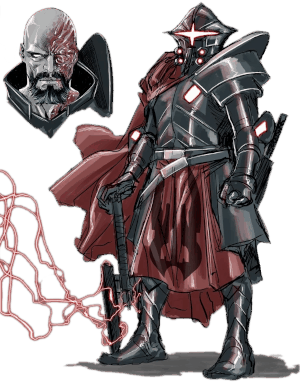
\includegraphics[width=\linewidth]{_img/pnjs/bombinax.png}
\caption{\nameref{sec:bombinax}}
\end{figure}

Selon le niveau et le nombre de vos héros, vous pouvez ajouter des \nameref{sec:citadel-guard} pour équilibrer.
\bigbreak
Le combat terminé, les héros finissent de se rendre à la terrasse du niveau 18 pour y retrouver \nameref{sec:aphra}.
\newpage

\subsection{Terrassé}

Vos héros arrivent donc dans la salle de réception qu’ils connaissent déjà. De l’autre côté de la pièce, sur la terrasse, \nameref{sec:aphra} les appelle. On peut voir son vaisseau derrière elle en vol stationnaire.

\begin{quotebox}
\noindent\textbf{\nameref{sec:aphra}}: Allez, grouillez-vous !
\end{quotebox}

Dès que les héros s’avancent, ils voient, sortir de derrière une colonne juste à côté d’\nameref{sec:aphra}, la \nameref{sec:ktath-atn-queen} en personne arborant un large sourire. Derrière les héros, les portes de la salle se referment et une dizaine de \nameref{sec:citadel-guard} sortent de nulle part et les encercle. C’est enfin au tour de \nameref{sec:varroa} et \nameref{sec:vespinax} de se montrer. Bref, les héros n’ont aucune chance de s’en tirer.

\begin{quotebox}
\noindent\textbf{\nameref{sec:ktath-atn-queen}}: Vous avez rempli votre part du marché Aphra, donnez-moi le cristal.
\end{quotebox}
La reine prend le cristal dans ces mains, le manipule un moment, le cristal s’illumine brièvement, puis la reine le rend à Aphra.
\begin{quotebox}
\noindent\textbf{\nameref{sec:ktath-atn-queen}}: Tenez, maintenant quittez ma planète et n’y revenez plus.\\
\noindent\textbf{\nameref{sec:aphra}}: Que va-t-il leur arriver maintenant ?\\
\noindent\textbf{\nameref{sec:ktath-atn-queen}}: \nameref{sec:varroa}, assure-toi qu’elle quitte la planète immédiatement\\
\noindent\textbf{\nameref{sec:varroa}}: Bien-sur ma reine.
\end{quotebox}
\nameref{sec:varroa} fait signe à \nameref{sec:aphra} de passer devant et tout deux montent dans le vaisseau.
\begin{quotebox}
\noindent\textbf{\nameref{sec:aphra}}: Vous comptez retourner sur Horox III avec moi ?\\
\noindent\textbf{\nameref{sec:varroa}}: Vous n’aurez qu’à me laisser sur la station orbitale.
\end{quotebox}
La soute du vaisseau se referme et le vaisseau s’éloigne vers l’espace.

\begin{quotebox}
\noindent\textbf{\nameref{sec:ktath-atn-queen}}: \nameref{sec:vespinax}, si l’un d’eux n’est pas compatible avec les symbiotes, tue-le. Pour les autres prépare les et amène les moi dans mes quartiers.\\
\noindent\textbf{\nameref{sec:vespinax}}: Bien ma reine.
\end{quotebox}
La reine sort nonchalamment de la salle de réception. C’est alors que des \nameref{sec:symbiote-abersyn}s tombent du plafond et se dirigent vers les héros. En plus de \nameref{sec:vespinax}, il reste encore 5 \textit{(mettre un peu moins de garde que de héros histoire d’équilibrer)} \nameref{sec:citadel-guard}.

Pour cette scène, faite jouer les \nameref{sec:symbiote-abersyn}s en un tour de jeux. Vous en faites attaquer avec \textbf{Bag}arre, s’il n’est pas paré et qu’il touche, il ne fera pas de dégât, mais le héros devra forcément attaquer le symbiote pour s’en débarrasser.

\nameref{sec:vespinax} n’a pas d’armure mais elle est très agile et donc difficile à toucher.

\begin{figure}[h]
\noindent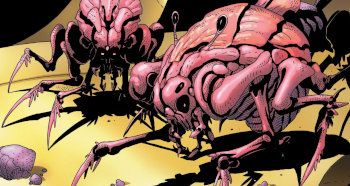
\includegraphics[width=\linewidth]{_img/bestiary/symbiote-abersyn.jpg}
\caption{\nameref{sec:symbiote-abersyn}}
\end{figure}
Dès que \nameref{sec:vespinax} est KO, un énorme vacarme retenti et le combat s’arrête. C’est le vaisseau \nameref{sec:aphra} qui vient de s’écraser dans la salle de réception, balayant au passage ce qu’il reste de symbiotes et de garde.
La soute s’ouvre \nameref{sec:aphra} à côté d’elle roule un droïde noir, la tête de \nameref{sec:varroa} est planté sur l’un de ses bras.

\begin{quotebox}
\noindent\textbf{\nameref{sec:aphra}}: BT-1, tu veux bien arrêter de jouer avec ça s’il te plaît !
\end{quotebox}
BT-1 fait des bips d’un air râleur et balance la tête par-dessus ce qu’il reste du balcon. \nameref{sec:aphra} se tourne alors vers nos héros.
\begin{quotebox}
\noindent\textbf{\nameref{sec:aphra}}: Bon ok, je sais c’est pas cool, mais elle aurait jamais accepté d’ouvrir l’artefact sans ça. J’ai jamais eu l’intention de vous laisser. Là maintenant vous êtes énervé mais prenez un peu de recul, vous verrez que c’était la seule solution. Et puis vous n’avez rien, tout va bien.
\end{quotebox}
Laissez les héros s’énerver un peu ou poser des questions\dots
\begin{quotebox}
\noindent\textbf{\nameref{sec:aphra}}: \'Ecoutez on pourrait remettre ça plus tard ? Il faut qu’on s’occupe de la reine. Ces espèces d’araignées, ce sont des \nameref{sec:symbiote-abersyn}s, un peu comme un bernard-l’hermite ces trucs quittent leur carapace et viennent se loger dans votre tête. Une fois en place, vous devenez un légume au service de la reine. Toute la population de cette planète est contaminé. Mais si on tue la reine, tous les symbiotes mourront instantanément. On ne peut pas laisser ces pauvres gens.
\end{quotebox}